\subsection{Benchmark functions}
In this paper, we compare the performance of the binary version of GA, PSO and HPSOWM that will be called BGA, BPSO, BHPSOWM respectively, using a suite of benchmark test functions (shown in \ref{table1}). Many different kinds of optimization problems are covered by these benchmark test functions \cite{ling2008hybrid}. They are divided into three categories as follows:
\begin{itemize}
	\item Category I - Unimodal functions: a symmetry model with a single minimum. Function $f_1$ to $f_7$ are in this category
	\item Category II - Multimodal functions with few local minima. Function $f_8$ to $f_{13}$ belong to this.
	\item Category III - Multimodal functions with many local minima which includes function $f_{14}$ to $f_{18}$
\end{itemize}


% Benchmark functions

\begin{table}[H]\label{table1}
	\caption{Benchmark test functions}
	\begin{center}
		\bgroup
		\def\arraystretch{1.5}%  1 is the default, change whatever you need
	    \begin{tabular}{  >{\centering\arraybackslash}m{8cm} | >{\centering\arraybackslash}m{3cm} | >{\centering\arraybackslash}m{3cm} }
		    \hline
		    Test function & Domain range & Optimal point \\ \hline
    
		    $f_1(x) = \sum\limits_{i=1}^{30}{x_i}^2$ & 
		    $-100 \leq x_i \leq 100$ & 
		    $f_i(0) = 0$ 
    			\\ \hline
    			
    			$f_2(x) = \sum\limits_{i=1}^{9}\Big[ 100(x_{i+1} - x_{i}^2)^2 + (x_i - 1)^2 \Big]$ &
    			$-2.048 \leq x_i \leq 2.048$ &
    			$f_2(1) = 0$    			
    			\\ \hline
    			
    			$f_3(x) = \sum\limits_{i=1}^{100}(|x_i + 0.5|)^2$ &
    			$-10 \leq x_i \leq 10$ &
    			$f_3(0) = 0$ 
    			\\ \hline    			
    			
    			$f_4(x) = \sum\limits_{i=1}^{10}ix_{i}^4 + random[0,1)$ &
    			$-2.56 \leq x_i \leq 2.56$ &
    			$f_4(0) = 0$
    			\\ \hline
    			
    			$f_5(x) = max{|x_i|, 1 \leq i \leq 30}$ &
    			$-100 \leq x_i \leq 100$ &
    			$f_5(0) = 0$
    			\\ \hline
    			
    			$f_6(x) = \sum\limits_{i=1}^{30}|x_i| + \prod\limits_{i=1}^{30}|x_i|$ &
    			$-10 \leq x_i \leq 10$ &
    			$f_5(0) = 0$
    			\\ \hline
    			
    			
    			$f_7(x) = -cos(x_1) \cdot cos(x_2) \cdot exp \Big( -\Big( (x_1 - \pi)^2 + (x_2 + \pi)^2\Big) \Big)$ &
    			$-300 \leq x_1, x_2 \leq 300$ &
    			$f_7(\Big[ \pi,\pi \Big]) = -1$
    			\\ \hline
    			
    			$f_8(x) = \Bigg[ \frac{1}{500} + \sum\limits_{j=1}^{25}\frac{1}{j + \sum_{i=1}^{2}(x_i - a_{ij})^6} \Bigg]^{-1}$ &
    			$-65.536 \leq x_1, x_2 \leq 65.536$ &
    			$f_8(|-32, 32|) \approx 1$
    			\\ \hline
    			
    			$f_9(x) = \sum\limits_{i=1}^{9} \Bigg[ a_i - \frac{x_1(b_{i}^2 + b_i x_2)}{b_{i}^2 + b_i x_3 + x_4} \Bigg]^2$ &
    			$-5 \leq x_i \leq 5$ &
    			$f_9(0.1928, 0.1928, 0.1231, 0.1358) \approx 0.0003075$
    			\\ \hline
    			
    			$f_{10}(x) = -\frac{sin(x_1)sin(x_2)}{x_1 x_2}$ &
    			$-10 \leq x_1, x_2 \leq 10$ &
    			$\displaystyle\lim_{x \to |0,0|}f_{10}(x) = -1$
    			\\ \hline
    			
    			$f_{11}(x) = 4x_{1}^2 - 2.1x_{1}^4 + \frac{1}{3}x_{1}^6 + x_1 x_2 - 4x_{2}^2 + 4x_{2}^4$ &
    			$-5 \leq x_1, x_2 \leq 5$ &
    			$f_{11}(\Big[ 0.08983, -0.7126 \Big]) = f_{11}(\Big[ -0.08983, 0.7126 \Big]) \approx -1.0316$
    			\\ \hline
    			
    			$f_{12}(x) = -\sum\limits_{i=1}^{30}c_i exp\Bigg[ -\sum\limits_{j=1}^{3}a_{ij}\Big( x_j - p_{ij} \Big)^2 \Bigg]$ &
    			$0 \leq x_i \leq 1$ &
    			$f_{12}(0.114, 0.556, 0.852) \approx -3.8628$
    			\\ \hline
    			
    			$f_{13}(x) = -\sum\limits_{i=1}^{4}c_i exp\Bigg[ -\sum\limits_{j=1}^{6}a_{ij}\Big( x_j - p_{ij} \Big)^2 \Bigg]$ &
    			$0 \leq x_i \leq 1$ &
    			$f_{13}(\Big[ 0.201, 0.15, 0.477, 0.275, 0.311, 0.627 \Big]) \approx -3.32$
    			\\ \hline
    			
			$
			f_{14}(x) = 0.1 \left\{ \begin{array}{l}
        			sin^2(\pi 3 x_1) \\
        			+ \sum\limits_{i=1}^{29}(x_i - 1)^2 \cdot \Big[ 1 + sin^2(3 \pi x_{i+1}) \Big] \\
        			+ (x_30 - 1)^2 \Big[ 1 + sin^2(2 \pi x_30) \Big]
    			\end{array}\right\}    		
    			+ \sum\limits_{i=1}^{30}u(x_i, 5, 100, 4)
			$ &
			$-50 \leq x_i \leq 50$ &
			$f_{14}(1) = 0$
			\\ \hline
			
			$f_{15}(x) = \sum\limits_{i=1}^{30}\Bigg[ x_{i}^2 - 10 cos(2\pi x_i) + 10 \Bigg]$ &
			$-50 \leq x_i \leq 50$ &
			$f_{15}(0) = 0$
			\\ \hline
			
			$f_{16}(x) = \frac{1}{4000}\sum\limits_{i=1}^{30}x_{i}^2 - \prod_{i=1}^{30}cos\Bigg( \frac{x_i}{\sqrt{i}} \Bigg) + 1$ &
			$-600 \leq x_i \leq 600$ &
			$f_{16}(0) = 0$
			\\ \hline
			
			$f_{17}(x) = -20exp \Bigg( -0.2\sqrt{\frac{1}{30}\sum\limits_{i=1}^{30}x_{i}^2} \Bigg) - exp \Bigg( \frac{1}{30} \sum\limits_{i=1}^{30}cos 2 \pi x_i \Bigg) + 20 + e$ &
			$-32 \leq x_i \leq 32$ &
			$f_{17}(0) = 0$
			\\ \hline
			
			$f_{18}(x) = -\sum\limits_{i=1}^{10}\Bigg( x_i sin\Bigg( \sqrt{|x_i|} \Bigg) \Bigg)$ &
			$-500 \leq x_i \leq 500$ &
			$f_{18}([420.9687, \cdots 420.9687]) = -10 \times 418.9829 = -4189.829$
			\\ \hline
    			
    		\end{tabular}
    		\egroup
	\end{center}
\end{table}

\subsection{Experiment settings}
We adapt the settings from the original research of HPSOWM \cite{ling2008hybrid} which has some main settings are:
\begin{itemize}
	\item Swarm size: 50
	\item Number of runs: 50
	\item Time limit for each run: 120 seconds
	\item The probability of crossover for GA: 0.001
	\item The initial population: we start from a single initial population so we can compare the performance among three algorithms starting from the same point
\end{itemize}
As of the binary version, we also adapt the settings from \cite{kennedy1997discrete} as:
\begin{itemize}
	\item $V_{max}$ which is the maximum value for the velocity is set to 6
\end{itemize}

\subsection{Results and Discussions}

- Compare BHPSOWM with BPSO and GA \\
- Use benchmark functions in three categories: unimodal functions, multimodal functions with few local minima, multimodal functions with many local minima \\
- Experiment settings \\
- Show convergence table \\
- Show result table with Standard Deviation, ... \\



\begin{table}[H]
\caption{Comparison between BHPSOWM, BPSO and GA - Category I: unimodal functions}\label{tab:graph1}
  \begin{tabular*}{\textwidth}{cc}
    \begin{tabular}[c]{@{}c@{}}
    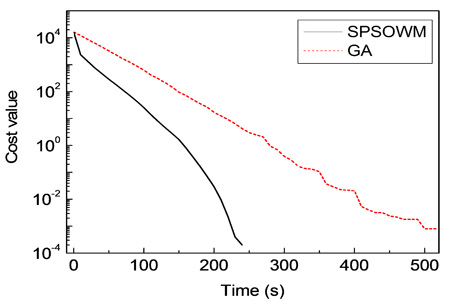
\includegraphics[width=60mm]{resources/f1x} \\
    $f_1(x)$
    \end{tabular}
    &
    \begin{tabular}[c]{@{}c@{}}
    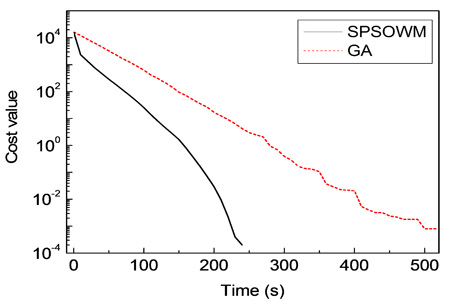
\includegraphics[width=60mm]{resources/f1x} \\
    $f_2(x)$
    \end{tabular}
    \\
    \begin{tabular}[c]{@{}c@{}}
    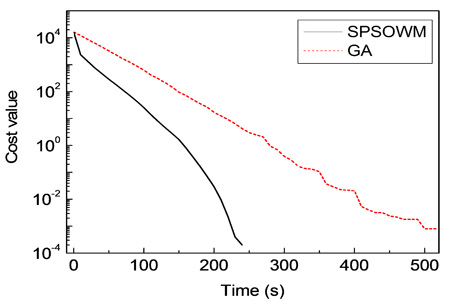
\includegraphics[width=60mm]{resources/f1x} \\
    $f_3(x)$
    \end{tabular}
    &
    \begin{tabular}[c]{@{}c@{}}
    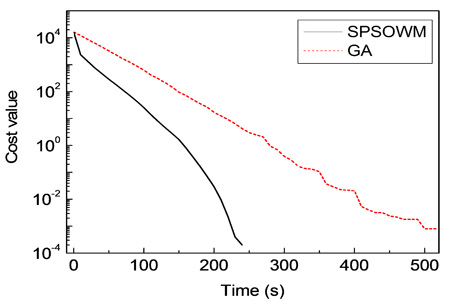
\includegraphics[width=60mm]{resources/f1x} \\
    $f_4(x)$
    \end{tabular}
    \\
    \begin{tabular}[c]{@{}c@{}}
    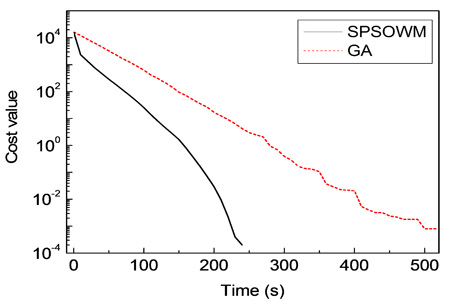
\includegraphics[width=60mm]{resources/f1x} \\
    $f_5(x)$
    \end{tabular}
    &

    \\
  \end{tabular*}
\end{table}


\begin{table}[H]
\caption{Comparison between BHPSOWM, BPSO and GA - Category II: multimodal functions with few local minima}\label{tab:graph2}
  \begin{tabular*}{\textwidth}{cc}
    \begin{tabular}[c]{@{}c@{}}
    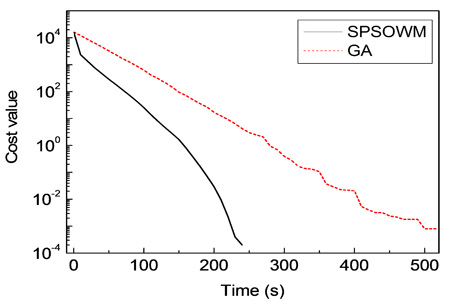
\includegraphics[width=60mm]{resources/f1x} \\
    $f_1(x)$
    \end{tabular}
    &
    \begin{tabular}[c]{@{}c@{}}
    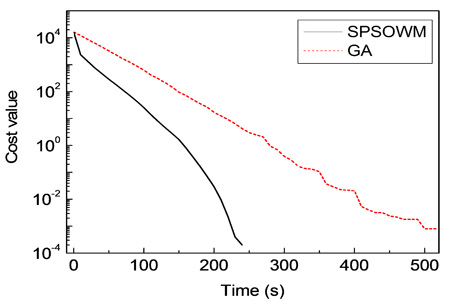
\includegraphics[width=60mm]{resources/f1x} \\
    $f_2(x)$
    \end{tabular}
    \\
    \begin{tabular}[c]{@{}c@{}}
    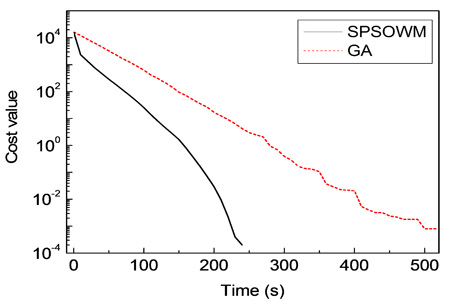
\includegraphics[width=60mm]{resources/f1x} \\
    $f_3(x)$
    \end{tabular}
    &
    \begin{tabular}[c]{@{}c@{}}
    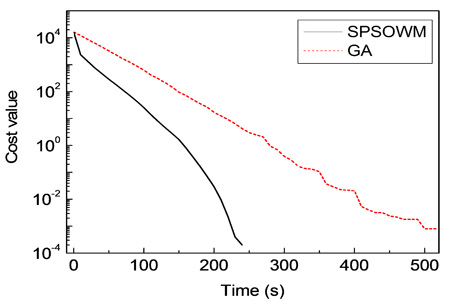
\includegraphics[width=60mm]{resources/f1x} \\
    $f_4(x)$
    \end{tabular}
    \\
    \begin{tabular}[c]{@{}c@{}}
    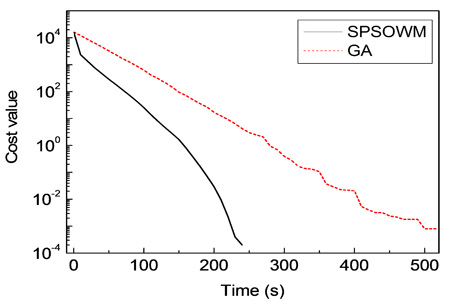
\includegraphics[width=60mm]{resources/f1x} \\
    $f_5(x)$
    \end{tabular}
    &

    \\
  \end{tabular*}
\end{table}


\begin{table}[H]
\caption{Comparison between BHPSOWM, BPSO and GA - Category III: multimodal functions with many local minima}\label{tab:graph3}
  \begin{tabular*}{\textwidth}{cc}
    \begin{tabular}[c]{@{}c@{}}
    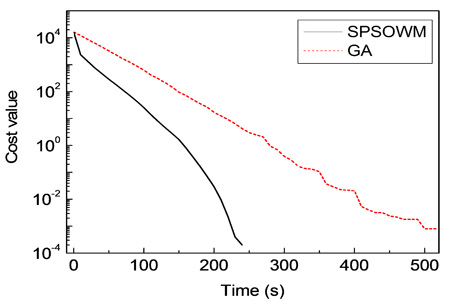
\includegraphics[width=60mm]{resources/f1x} \\
    $f_1(x)$
    \end{tabular}
    &
    \begin{tabular}[c]{@{}c@{}}
    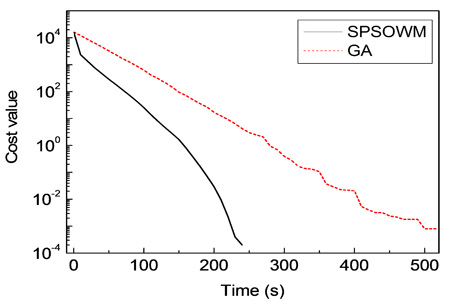
\includegraphics[width=60mm]{resources/f1x} \\
    $f_2(x)$
    \end{tabular}
    \\
    \begin{tabular}[c]{@{}c@{}}
    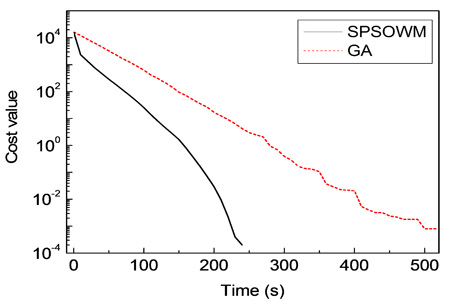
\includegraphics[width=60mm]{resources/f1x} \\
    $f_3(x)$
    \end{tabular}
    &
    \begin{tabular}[c]{@{}c@{}}
    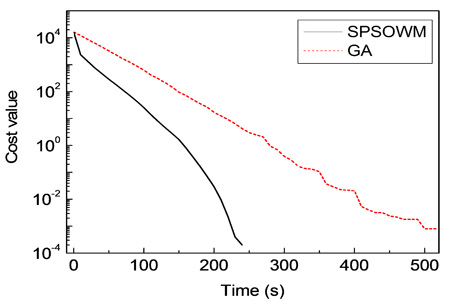
\includegraphics[width=60mm]{resources/f1x} \\
    $f_4(x)$
    \end{tabular}
    \\
    \begin{tabular}[c]{@{}c@{}}
    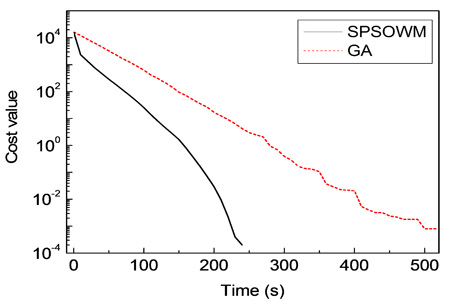
\includegraphics[width=60mm]{resources/f1x} \\
    $f_5(x)$
    \end{tabular}
    &

    \\
  \end{tabular*}
\end{table}





\renewcommand{\arraystretch}{1}
\setlength{\tabcolsep}{.1em}
\begin{table}[H]
\caption{Comparison between BHPSOWM, BPSO and GA with benchmark testing function - Category I}\label{tab:tb2}
\centering
  \begin{tabular}{|c|l|r|r|r|}
  \hline
  & & BHPSOWM & BPSO & GA \\
  \hline
  
  % begin function
  \begin{tabular}[c]{@{}c@{}}
  $f_1(x)$\\
  $T = 120$
  \end{tabular}
  &
  \begin{tabular}[c]{@{}lll@{}}
  Best\\
  Mean\\
  Std Dev
  \end{tabular}
  &
  \begin{tabular}{@{}rrr@{}}
  0.000\\
  0.000\\
  0.000
  \end{tabular}
  &
  \begin{tabular}{@{}rrr@{}}
  0.000\\
  0.000\\
  0.000
  \end{tabular} 
  &
  \begin{tabular}{@{}rrr@{}}
  0.000\\
  0.000\\
  0.000
  \end{tabular} 
  \\ \hline
  % end of function 
  
  % begin function
  \begin{tabular}[c]{@{}c@{}}
  $f_2(x)$\\
  $T = 120$
  \end{tabular}
  &
  \begin{tabular}[c]{@{}lll@{}}
  Best\\
  Mean\\
  Std Dev
  \end{tabular}
  &
  \begin{tabular}{@{}rrr@{}}
  0.000\\
  0.000\\
  0.000
  \end{tabular}
  &
  \begin{tabular}{@{}rrr@{}}
  0.000\\
  0.000\\
  0.000
  \end{tabular} 
  &
  \begin{tabular}{@{}rrr@{}}
  0.000\\
  0.000\\
  0.000
  \end{tabular} 
  \\ \hline
  % end of function 
  
  % begin function
  \begin{tabular}[c]{@{}c@{}}
  $f_3(x)$\\
  $T = 120$
  \end{tabular}
  &
  \begin{tabular}[c]{@{}lll@{}}
  Best\\
  Mean\\
  Std Dev
  \end{tabular}
  &
  \begin{tabular}{@{}rrr@{}}
  0.000\\
  0.000\\
  0.000
  \end{tabular}
  &
  \begin{tabular}{@{}rrr@{}}
  0.000\\
  0.000\\
  0.000
  \end{tabular} 
  &
  \begin{tabular}{@{}rrr@{}}
  0.000\\
  0.000\\
  0.000
  \end{tabular} 
  \\ \hline
  % end of function 
  
  % begin function
  \begin{tabular}[c]{@{}c@{}}
  $f_4(x)$\\
  $T = 120$
  \end{tabular}
  &
  \begin{tabular}[c]{@{}lll@{}}
  Best\\
  Mean\\
  Std Dev
  \end{tabular}
  &
  \begin{tabular}{@{}rrr@{}}
  0.000\\
  0.000\\
  0.000
  \end{tabular}
  &
  \begin{tabular}{@{}rrr@{}}
  0.000\\
  0.000\\
  0.000
  \end{tabular} 
  &
  \begin{tabular}{@{}rrr@{}}
  0.000\\
  0.000\\
  0.000
  \end{tabular} 
  \\ \hline
  % end of function 
  
  % begin function
  \begin{tabular}[c]{@{}c@{}}
  $f_5(x)$\\
  $T = 120$
  \end{tabular}
  &
  \begin{tabular}[c]{@{}lll@{}}
  Best\\
  Mean\\
  Std Dev
  \end{tabular}
  &
  \begin{tabular}{@{}rrr@{}}
  0.000\\
  0.000\\
  0.000
  \end{tabular}
  &
  \begin{tabular}{@{}rrr@{}}
  0.000\\
  0.000\\
  0.000
  \end{tabular} 
  &
  \begin{tabular}{@{}rrr@{}}
  0.000\\
  0.000\\
  0.000
  \end{tabular} 
  \\ \hline
  % end of function 
  
  % begin function
  \begin{tabular}[c]{@{}c@{}}
  $f_6(x)$\\
  $T = 120$
  \end{tabular}
  &
  \begin{tabular}[c]{@{}lll@{}}
  Best\\
  Mean\\
  Std Dev
  \end{tabular}
  &
  \begin{tabular}{@{}rrr@{}}
  0.000\\
  0.000\\
  0.000
  \end{tabular}
  &
  \begin{tabular}{@{}rrr@{}}
  0.000\\
  0.000\\
  0.000
  \end{tabular} 
  &
  \begin{tabular}{@{}rrr@{}}
  0.000\\
  0.000\\
  0.000
  \end{tabular} 
  \\ \hline
  % end of function 
  
  % begin function
  \begin{tabular}[c]{@{}c@{}}
  $f_7(x)$\\
  $T = 120$
  \end{tabular}
  &
  \begin{tabular}[c]{@{}lll@{}}
  Best\\
  Mean\\
  Std Dev
  \end{tabular}
  &
  \begin{tabular}{@{}rrr@{}}
  0.000\\
  0.000\\
  0.000
  \end{tabular}
  &
  \begin{tabular}{@{}rrr@{}}
  0.000\\
  0.000\\
  0.000
  \end{tabular} 
  &
  \begin{tabular}{@{}rrr@{}}
  0.000\\
  0.000\\
  0.000
  \end{tabular} 
  \\ \hline
  % end of function  
  
  \end{tabular}
\end{table}










\renewcommand{\arraystretch}{1}
\setlength{\tabcolsep}{.1em}
\begin{table}[H]
\caption{Comparison between BHPSOWM, BPSO and GA with benchmark testing function - Category II}\label{tab:tb3}
\centering
  \begin{tabular}{|c|l|r|r|r|}
  \hline
  & & BHPSOWM & BPSO & GA \\
  \hline
  
  % begin function
  \begin{tabular}[c]{@{}c@{}}
  $f_8(x)$\\
  $T = 120$
  \end{tabular}
  &
  \begin{tabular}[c]{@{}lll@{}}
  Best\\
  Mean\\
  Std Dev
  \end{tabular}
  &
  \begin{tabular}{@{}rrr@{}}
  0.000\\
  0.000\\
  0.000
  \end{tabular}
  &
  \begin{tabular}{@{}rrr@{}}
  0.000\\
  0.000\\
  0.000
  \end{tabular} 
  &
  \begin{tabular}{@{}rrr@{}}
  0.000\\
  0.000\\
  0.000
  \end{tabular} 
  \\ \hline
  % end of function  
  
  % begin function
  \begin{tabular}[c]{@{}c@{}}
  $f_9(x)$\\
  $T = 120$
  \end{tabular}
  &
  \begin{tabular}[c]{@{}lll@{}}
  Best\\
  Mean\\
  Std Dev
  \end{tabular}
  &
  \begin{tabular}{@{}rrr@{}}
  0.000\\
  0.000\\
  0.000
  \end{tabular}
  &
  \begin{tabular}{@{}rrr@{}}
  0.000\\
  0.000\\
  0.000
  \end{tabular} 
  &
  \begin{tabular}{@{}rrr@{}}
  0.000\\
  0.000\\
  0.000
  \end{tabular} 
  \\ \hline
  % end of function  
  
  % begin function
  \begin{tabular}[c]{@{}c@{}}
  $f_10(x)$\\
  $T = 120$
  \end{tabular}
  &
  \begin{tabular}[c]{@{}lll@{}}
  Best\\
  Mean\\
  Std Dev
  \end{tabular}
  &
  \begin{tabular}{@{}rrr@{}}
  0.000\\
  0.000\\
  0.000
  \end{tabular}
  &
  \begin{tabular}{@{}rrr@{}}
  0.000\\
  0.000\\
  0.000
  \end{tabular} 
  &
  \begin{tabular}{@{}rrr@{}}
  0.000\\
  0.000\\
  0.000
  \end{tabular} 
  \\ \hline
  % end of function  
  
  % begin function
  \begin{tabular}[c]{@{}c@{}}
  $f_11(x)$\\
  $T = 120$
  \end{tabular}
  &
  \begin{tabular}[c]{@{}lll@{}}
  Best\\
  Mean\\
  Std Dev
  \end{tabular}
  &
  \begin{tabular}{@{}rrr@{}}
  0.000\\
  0.000\\
  0.000
  \end{tabular}
  &
  \begin{tabular}{@{}rrr@{}}
  0.000\\
  0.000\\
  0.000
  \end{tabular} 
  &
  \begin{tabular}{@{}rrr@{}}
  0.000\\
  0.000\\
  0.000
  \end{tabular} 
  \\ \hline
  % end of function  
  
  % begin function
  \begin{tabular}[c]{@{}c@{}}
  $f_12(x)$\\
  $T = 120$
  \end{tabular}
  &
  \begin{tabular}[c]{@{}lll@{}}
  Best\\
  Mean\\
  Std Dev
  \end{tabular}
  &
  \begin{tabular}{@{}rrr@{}}
  0.000\\
  0.000\\
  0.000
  \end{tabular}
  &
  \begin{tabular}{@{}rrr@{}}
  0.000\\
  0.000\\
  0.000
  \end{tabular} 
  &
  \begin{tabular}{@{}rrr@{}}
  0.000\\
  0.000\\
  0.000
  \end{tabular} 
  \\ \hline
  % end of function  
  
  % begin function
  \begin{tabular}[c]{@{}c@{}}
  $f_13(x)$\\
  $T = 120$
  \end{tabular}
  &
  \begin{tabular}[c]{@{}lll@{}}
  Best\\
  Mean\\
  Std Dev
  \end{tabular}
  &
  \begin{tabular}{@{}rrr@{}}
  0.000\\
  0.000\\
  0.000
  \end{tabular}
  &
  \begin{tabular}{@{}rrr@{}}
  0.000\\
  0.000\\
  0.000
  \end{tabular} 
  &
  \begin{tabular}{@{}rrr@{}}
  0.000\\
  0.000\\
  0.000
  \end{tabular} 
  \\ \hline
  % end of function  
  
  \end{tabular}
\end{table}













\renewcommand{\arraystretch}{1}
\setlength{\tabcolsep}{.1em}
\begin{table}[H]
\caption{Comparison between BHPSOWM, BPSO and GA with benchmark testing function - Category III}\label{tab:tb4}
\centering
  \begin{tabular}{|c|l|r|r|r|}
  \hline
  & & BHPSOWM & BPSO & GA \\
  \hline
  
  % begin function
  \begin{tabular}[c]{@{}c@{}}
  $f_14(x)$\\
  $T = 120$
  \end{tabular}
  &
  \begin{tabular}[c]{@{}lll@{}}
  Best\\
  Mean\\
  Std Dev
  \end{tabular}
  &
  \begin{tabular}{@{}rrr@{}}
  0.000\\
  0.000\\
  0.000
  \end{tabular}
  &
  \begin{tabular}{@{}rrr@{}}
  0.000\\
  0.000\\
  0.000
  \end{tabular} 
  &
  \begin{tabular}{@{}rrr@{}}
  0.000\\
  0.000\\
  0.000
  \end{tabular} 
  \\ \hline
  % end of function  
  
  
  % begin function
  \begin{tabular}[c]{@{}c@{}}
  $f_15(x)$\\
  $T = 120$
  \end{tabular}
  &
  \begin{tabular}[c]{@{}lll@{}}
  Best\\
  Mean\\
  Std Dev
  \end{tabular}
  &
  \begin{tabular}{@{}rrr@{}}
  0.000\\
  0.000\\
  0.000
  \end{tabular}
  &
  \begin{tabular}{@{}rrr@{}}
  0.000\\
  0.000\\
  0.000
  \end{tabular} 
  &
  \begin{tabular}{@{}rrr@{}}
  0.000\\
  0.000\\
  0.000
  \end{tabular} 
  \\ \hline
  % end of function  
  
  % begin function
  \begin{tabular}[c]{@{}c@{}}
  $f_16(x)$\\
  $T = 120$
  \end{tabular}
  &
  \begin{tabular}[c]{@{}lll@{}}
  Best\\
  Mean\\
  Std Dev
  \end{tabular}
  &
  \begin{tabular}{@{}rrr@{}}
  0.000\\
  0.000\\
  0.000
  \end{tabular}
  &
  \begin{tabular}{@{}rrr@{}}
  0.000\\
  0.000\\
  0.000
  \end{tabular} 
  &
  \begin{tabular}{@{}rrr@{}}
  0.000\\
  0.000\\
  0.000
  \end{tabular} 
  \\ \hline
  % end of function  
  
  % begin function
  \begin{tabular}[c]{@{}c@{}}
  $f_17(x)$\\
  $T = 120$
  \end{tabular}
  &
  \begin{tabular}[c]{@{}lll@{}}
  Best\\
  Mean\\
  Std Dev
  \end{tabular}
  &
  \begin{tabular}{@{}rrr@{}}
  0.000\\
  0.000\\
  0.000
  \end{tabular}
  &
  \begin{tabular}{@{}rrr@{}}
  0.000\\
  0.000\\
  0.000
  \end{tabular} 
  &
  \begin{tabular}{@{}rrr@{}}
  0.000\\
  0.000\\
  0.000
  \end{tabular} 
  \\ \hline
  % end of function  
  
  % begin function
  \begin{tabular}[c]{@{}c@{}}
  $f_18(x)$\\
  $T = 120$
  \end{tabular}
  &
  \begin{tabular}[c]{@{}lll@{}}
  Best\\
  Mean\\
  Std Dev
  \end{tabular}
  &
  \begin{tabular}{@{}rrr@{}}
  0.000\\
  0.000\\
  0.000
  \end{tabular}
  &
  \begin{tabular}{@{}rrr@{}}
  0.000\\
  0.000\\
  0.000
  \end{tabular} 
  &
  \begin{tabular}{@{}rrr@{}}
  0.000\\
  0.000\\
  0.000
  \end{tabular} 
  \\ \hline
  % end of function  
  \end{tabular}
\end{table}